% -*- mode: fundamental -*-

% ****************************************************************

\chapter{BSV: Modules and Interfaces; \\
Drum and Fife Interface and Module Skeleton}

\markboth{Ch \arabic{chapter}: CPU module skeleton; Modules, interfaces (DRAFT)}{\copyrightnotice}

\setcounter{page}{1}
% \renewcommand{\thepage}{\arabic{page}}
\renewcommand{\thepage}{\arabic{chapter}-\arabic{page}}

\label{ch_Module_Skeleton}

% ****************************************************************

\section{Introduction}

It is good engineering practice to organize the code for any
non-trivial system, whether in hardware or software, into a
well-structured network of smaller, manageable \emph{modules}.  Each
module should have a clear, independent specification so that it can
be understood on its own, and so that it can transparently be
substituted by another module with the same functionality but perhaps
other desirable properties ({\eg} speed, area, power).  The external
specification of a module---its ``interface''---should not rely on,
and ideally note even mention, internal implementation details of the
module.

For example, each of the units shown in
Figure~\ref{Fig_CPU_Module_Skeleton_Simple_Instr_Exec} could be a
separate module.
\begin{figure}[htbp]
  \centerline{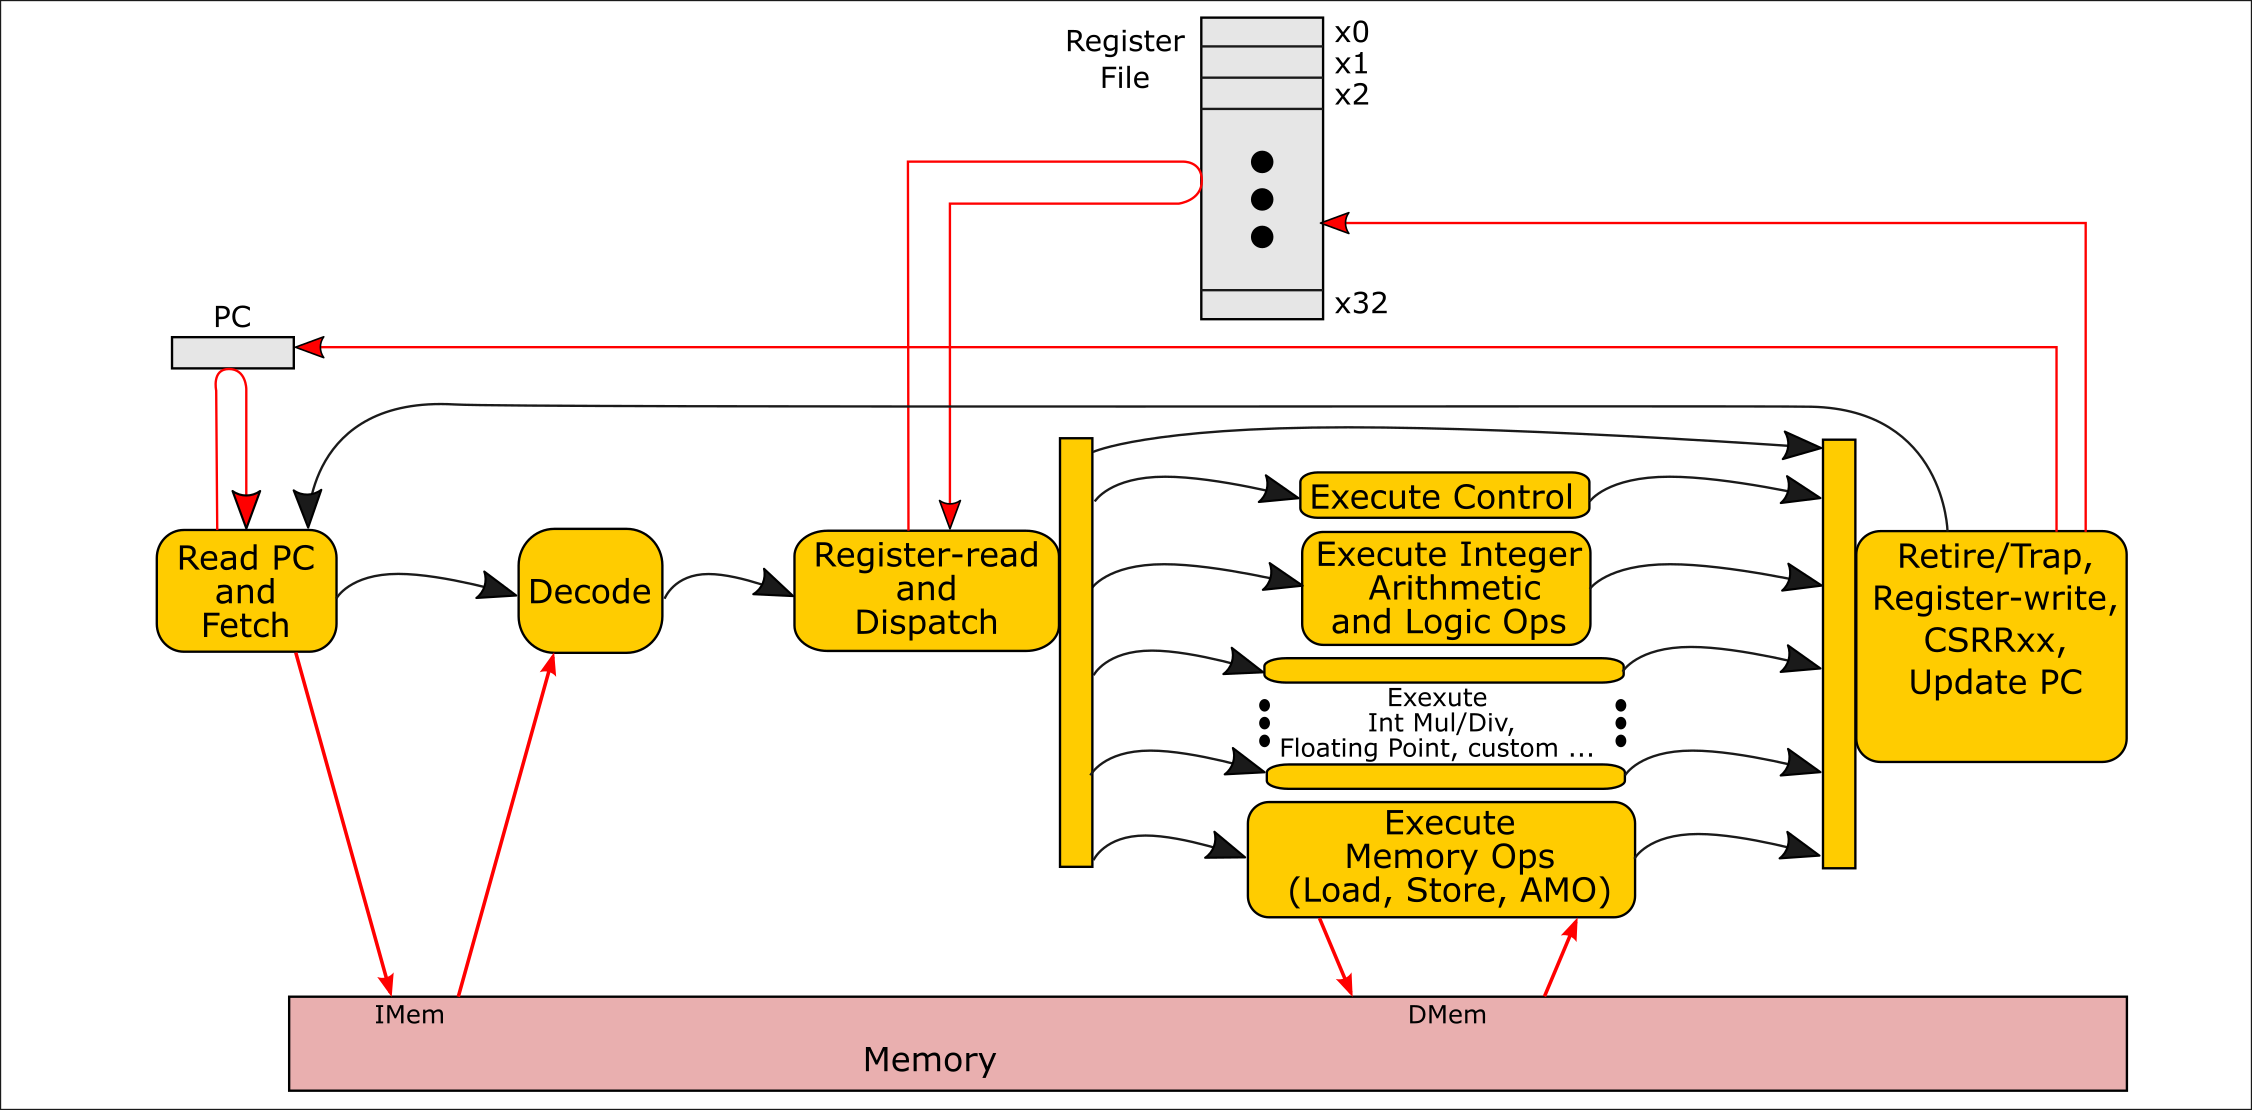
\includegraphics[width=6in,angle=0]{ch030_RISCV_Design_Space/Figures/Fig_Instr_Exec}}
  \caption{\label{Fig_CPU_Module_Skeleton_Simple_Instr_Exec}Simple interpretation of RISC-V instructions (same as Fig.~\ref{Fig_Instr_Exec})}
\end{figure}

In this chapter we discuss interfaces and modules in BSV, including a
few that are provided by the BSV libraries and are useful in
implementing our RISC-V CPUs.  At the end of this chapter, we show the
interface for the Drum and Fife CPUs---everything excluding the
Memory in Figure~\ref{Fig_CPU_Module_Skeleton_Simple_Instr_Exec}.

% ****************************************************************

\section{BSV: Modules: state, behavior and interfaces}

\label{Sec_CPU_Module_Skeleton_Modules}

\index{BSV!Module}

Modules encapsulate modifiable state, internal behavior (\emph{rules})
and external behavior (\emph{interface methods}).  In this sense they
are similar to ``objects'' in object-oriented programming languages
such as C++, Java, and Python.  A BSV module is like an object
constructor; a module \emph{instance} is like an object; and its
interface is \emph{a set of methods} that can be invoked like
functions/procedures.

Modules and interfaces clearly separate the concerns of
externally-visible functionality (``external API'', \emph{what} a
module does) {\vs} internal implementation details (\emph{how} the
module does it).

BSV modules are typically organized in a \emph{hierarchy}---in
Drum and Fife, the top-level system will be a module,
instantiating, as sub-modules, a CPU module (Drum or Fife) and a
memory system module; the CPU module, in turn, will instantiate
sub-modules such as a register-file module, and so on.  A clean,
common interface allows us transparently to substitute the Drum
CPU module for the Fife CPU module and \emph{vice versa}.

In the next several sections we describe the concepts of BSV modules
and interfaces.  These sections may require re-reading a couple of
times; the concepts become properly internalized only after
seeing/using/creating several examples.  Temporal behavior will be
discussed in the next chapter.

% ================================================================

\subsection{BSV: Interface declarations}

\index{BSV!Interface!type}
\index{BSV!Types!interface}

An \emph{interface declaration} in BSV declares a new interface, and
looks like this:

\begin{quote}
{\tt interface} \emph{interface-type};

\hmm \emph{... method and sub-interface declarations ...}

{\tt endinterface}
\end{quote}

The interface represents the external view of a module, {\ie} it
declares a set of \emph{methods} that can be invoked from an external
context.  Each method declaration only lists its arguments and their
types, and the method's overall result type.  The \emph{body} of the
method is defined elsewhere, within a specific module that offers this
interface type.

Interfaces can be nested (can contain sub-interfaces which themselves
have methods or sub-sub-interfaces, and so on).  This is just a
syntactic abstraction mechanism; ultimately, all interactions with a
module are through its methods, whether at the top level of the
interface type, in a sub-interface, in a sub-sub-interface, {\etc}

An \verb|interface| declaration just defines a new type.  There can be
any number of module declarations each of which offers the same
interface.  For example, the BSV library contains a repertoire of FIFO
modules, all of which have the same FIFO interface type.

Section~\ref{Sec_CPU_Module_Skeleton_Register_interface} shows the
interface declaration type for register modules.
Section~\ref{Sec_CPU_Module_Skeleton_FIFOF_interface} shows the
interface declaration type for FIFO modules.

% ================================================================

\subsection{BSV: Module declarations}

\label{Sec_CPU_Module_Skeleton_module_declarations}

\index{BSV!Module!state}
\index{BSV!Module!behavior}
\index{BSV!Module!interface}

A \emph{module declaration} in BSV describes a module with a
particular interface type:

\begin{quote}
{\tt (* synthesize *)} \\
{\tt module} \emph{module-name} {\tt (} \emph{interface-type} {\tt );}

\hmm \emph{... instantiation of module state (registers, FIFOs, other sub-modules) ...}

\hmm \emph{... behavior (rules and FSMs) ...}

\hmm \emph{... interface (API) method implementations ...}

{\tt endmodule}
\end{quote}

\index{BSV!synthesize@{\tt (* synthesize *)} attribute}

The \verb|(* synthesize *)| attribute at the top has no semantic
significance.  It is merely an indication to the \emph{bsc} compiler,
when compiling to Verilog, to create a Verilog module for this BSV
module, and not to ``inline'' it into any parent module.

\index{BSV!Module!instance}

A module declaration declares a module constructor; it can be invoked
multiple times to obtain multiple \emph{instances}.

% ****************************************************************

\section{BSV: Example: Registers}

\index{BSV!Register}

BSV treats all ``state elements'' (components that store persistent
values) uniformly as modules with interfaces.  This includes
``primitives'' like ordinary registers.

A register is the simplest storage element in digital hardware, a
single memory cell containing a single value (represented as a
bit-vector).  We can (over-)write with a new value, and we can read
out the value stored by the most recent write.

% ================================================================

\subsection{BSV: {\tt Reg\#(}\emph{t}{\tt )}, the register interface}

\label{Sec_CPU_Module_Skeleton_Register_interface}

\index{BSV!Interface!Reg@{\tt Reg} register interface}
\index{BSV!Register!Reg@{\tt Reg} register interface}
\index{BSV!Register!read@{\tt \_read} method}
\index{BSV!Register!write@{\tt \_write} method}

The standard register interface type in BSV has two methods:

\begin{Verbatim}[frame=single, numbers=left]
interface Reg #(t);
   method t _read();
   method Action _write (t x);
endinterface
\end{Verbatim}

Here, ``\verb|t|'' is the type of value stored in the register
(discussed in more detail below).

The \verb|_read()| method (with no arguments) just returns the value
stored in the register, of type \verb|t|.  The \verb|_write()| method
takes one argument, a value of type \verb|t|, and stores it in the
register, over-writing any previous value and holding the new value
until over-written by the next \verb|_write()|.

% ================================================================

\subsection{BSV: {\tt mkReg(}\emph{v}{\tt )}, a register module (consructor)}

\index{BSV!Module!mkReg@{\tt mkReg} module (constructor)}

\index{BSV!Register!mkReg@{\tt mkReg}!module (constructor)}
\index{BSV!mkReg@{\tt mkReg}!module (constructor)}

\index{BSV!Register!mkReg@{\tt mkReg}!reset value}
\index{BSV!mkReg@{\tt mkReg}!reset value}

A standard BSV library register module is \verb|mkReg|.  It is used to
instantiate a new register, with a specified reset value, using a
statement like this:

\index{BSV!Register!mkReg@{\tt mkReg}!instantiation}
\index{BSV!mkReg@{\tt mkReg}!instantiation}

\begin{Verbatim}[frame=single, numbers=left]
    Reg #(Bit #(XLEN)) pc <- mkReg (0);
\end{Verbatim}

Here we declare a new identifier \verb|pc| with interface type
\verb|Reg#(Bit#(XLEN))| (the register interface type) and bind it to
the interface offered by a newly instantiated register.  The ``0''
argument to \verb|mkReg()| specifies the reset-value of the register,
{\ie} the value held in the register immediately after the hardware
has been reset.

\index{BSV!Module!instantiation}

In general any module is instantiated using this syntax:

\begin{quote}
\emph{interface-type} \hm \emph{module-name} \hm {\tt <-} \hm \emph{module-constructor};
\end{quote}

Different module-constructors may or may not have arguments.  For
example, this instantiation uses a different BSV library register
constructor:

\index{BSV!Register!mkRegU@{\tt mkRegU}!module (constructor)}
\index{BSV!mkRegU@{\tt mkRegU}!module (constructor)}

\begin{Verbatim}[frame=single, numbers=left]
   Reg #(Bit #(XLEN)) pc <- mkRegU;
\end{Verbatim}

\verb|mkRegU| instantiates a register with an unspecified
(unpredictable) reset value, and hence does not need an argument.

% ================================================================

\subsection{BSV: Registers are strongly typed}

\index{Register!strongly-typed}

Unlike Verilog and SystemVerilog, BSV registers are ``strongly
typed''.  Each register instance can only hold values of one
particular type.

Further, the register-contents type need not be \verb|Bits#()|; it can
more generally it can be \emph{any} BSV type that has a representation
in bits.  Thus, the type of a value in a register can be an enum, a
struct, a nested struct, {\etc}, if we have used a
\verb|deriving(Bits)| declaration (or its explicit analog) to ensure
that it has a representation in bits.

% ================================================================

\subsection{BSV: Syntactic shorthands for register access}

\label{Sec_CPU_Module_Skeleton_register_syntactic_shorthands}

\label{}

\index{Register!{\tt <=} register assignment}
\index{Register!implicit register read}

Registers are so ubuiquitous in digital design that BSV provides some
special syntactic shorthands for reading and writing registers.

Just mentioning a register in an expression can be used as a shorthand
for invoking its \verb|_read| method.  Thus, the expression:

\begin{Verbatim}[frame=single, numbers=left]
    rg_pc + 4
\end{Verbatim}

is shorthand for:

\begin{Verbatim}[frame=single, numbers=left]
    rg_pc._read + 4
\end{Verbatim}

To invoke the \verb|_write| method on a register, one can use a
conventional assignment statement.  Thus, the expression:

\begin{Verbatim}[frame=single, numbers=left]
    rg_pc._write (v)
\end{Verbatim}

can be written like this:\footnote{Rather than use ``{\tt =}'' or
``{\tt :=}'' common in software programming languages, we use ``{\tt
<=}'', which is the Verilog/SystemVerilog notation for ``delayed
assignment''.}

\begin{Verbatim}[frame=single, numbers=left]
    rg_pc <= v
\end{Verbatim}

To recap, a statement like this:

\begin{Verbatim}[frame=single, numbers=left]
    rg_pc <= rg_pc + 4
\end{Verbatim}

is shorthand for:

\begin{Verbatim}[frame=single, numbers=left]
    rg_pc._write (rg_pc_read + 4)
\end{Verbatim}

% ****************************************************************

\section{BSV: Example: FIFOs}

\index{BSV!FIFO}

FIFOs (First-in-First-out) elements are queues of values and are
broadly useful in any hardware design (arguably as useful as
registers).  We can enqueue a new value into a FIFO at the tail (back)
of the queue, and dequeue a value from the head (front) of the queue.
Most BSV FIFOs are automatically ``flow-controlled'', {\ie} it is
impossible to enqueue into a full FIFO and to dequeue from an empty
FIFO.

% ================================================================

\subsection{BSV: {\tt FIFOF\#(}\emph{t}{\tt )}, the FIFO interface}

\label{Sec_CPU_Module_Skeleton_FIFOF_interface}

\index{BSV!Interface!FIFOF@{\tt FIFOF} FIFO interface}
\index{BSV!FIFOF@{\tt FIFOF} interface}
\index{BSV!FIFOF@{\tt FIFOF}!type of stored value}
\index{BSV!FIFOF@{\tt FIFOF} interface methods}

A standard FIFO interface type in the BSV library is:

\begin{Verbatim}[frame=single, numbers=left]
interface FIFOF #(t);
   method Bool notEmpty();
   method Bool notFull();
   method t first();
   method Action deq();
   method Action enq (t x);
   method Action clear();
endinterface
\end{Verbatim}

Here, ``\verb|t|'' is the type of value stored in the register
(discussed in more detail below).

The \verb|notEmpty()| and \verb|notFull()| are simple predicates to
test if a FIFOF is empty or full, respectively.

The \verb|first()| and \verb|deq()| methods are used to access the
head of the queue.  They are only available if the FIFO is not empty.
The \verb|first()| method returns the value at the head of the queue.
This is non-destructive, {\ie} it does not modify the FIFO.  The
\verb|deq()| method modifies the FIFO: it discards the value at head
of the queue and advances the queue.

The \verb|enq()| method is used to access the tail of the queue, and
is only available if the FIFO is not full.  It modifies the FIFO by
appending the argument \verb|x| to the tail of the queue.

The \verb|clear| method is used to empty the queue immediately
(discard all its contents).

% ================================================================

\subsection{BSV: {\tt mkFIFOF}, a fifo module (constructor)}

\index{BSV!Module!mkFIFOF@{\tt mkFIFOF} module (constructor)}

\index{BSV!FIFO!mkFIFOF@{\tt mkFIFOF}!module (constructor)}
\index{BSV!FIFO!mkFIFOF@{\tt mkFIFOF}!reset value}
\index{BSV!mkFIFOF@{\tt mkFIFOF}!module (constructor)}
\index{BSV!mkFIFOF@{\tt mkFIFOF}!reset value}

The BSV library contains many different FIFO modules (constructors):
single-element FIFOs, FIFOs of a specified depth (queue length), FIFOs
with and without automatic flow-control, {\etc} In Drum we use
this one:

\index{BSV!FIFO!mkFIFOF@{\tt mkFIFOF}!instantiation}
\index{BSV!mkFIFOF@{\tt mkFIFOF}!instantiation}

\begin{Verbatim}[frame=single, numbers=left]
   FIFOF #(Mem_Req) f_to_IMem <- mkFIFOF;
\end{Verbatim}

Here we declare a new identifier \verb|f_to_IMem| with interface type
\verb|FIFOF#(Bit#(XLEN))| (the FIFO interface type) and bind it to the
interface offered by a newly instantiated FIFO.

Different module-constructors may or may not have arguments.  For
example, this instantiation uses a different BSV library FIFO
constructor:

\index{BSV!FIFO!mkSizedFIFOF@{\tt mkSizedFIFOF}!module (constructor)}
\index{BSV!mkSizedFIFOF@{\tt mkSizedFIFOF}!module (constructor)}

\begin{Verbatim}[frame=single, numbers=left]
   FIFOF #(RR_to_RW)  f_RR_to_RW  <- mkSizedFIFOF (8);
\end{Verbatim}

This instantiates a FIFOF of specific queue-depth (8).  Note that
module constructor arguments can play different roles.  In
\verb|mkReg| above, the argument (0) became a dynamic value, the value
held by the register after reset.  Here, the argument (8) only
describes \emph{structure}, {\ie} the size of the FIFO.

% ================================================================

\subsection{BSV: FIFOFs are strongly typed}

\index{FIFO!strongly-typed}

Each BSV FIFOF instance can only hold values of one particular type.

Further, the FIFO-contents type need not be \verb|Bits#()|; it can
more generally it can be \emph{any} BSV type that has a representation
in bits.  Thus, the type of values in a FIFO can be an enum, a struct,
a nested struct, {\etc}, if we have used a \verb|deriving(Bits)|
declaration (or its explicit analog) to ensure that it has a
representation in bits.

% ================================================================

\subsection{BSV: Semi-FIFO interfaces for each end of a FIFO}

FIFOs are often used to connect two separate modules together, for one
module to communicate values to the next one.  For example, the Fetch
step communicates memory requests to memory.  In this situation, one
module only interacts with the ``enqueue'' side, and the other module
only interacts with the ```dequeue'' side.

In these situations we will also find it useful to use the following
``Semi-FIFO'' interfaces interfaces for each ``end'' of a FIFO queue:

\index{BSV!FIFOF_O@{\tt FIFOF\_O}: semi-fifo interface}
\index{BSV!Semi-FIFO!{\tt FIFOF\_O} semi-fifo interface}

\begin{Verbatim}[frame=single, numbers=left]
interface FIFOF_O #(t);
   method Bool notEmpty();
   method t first();
   method Action deq();
endinterface
\end{Verbatim}

\index{BSV!FIFOF_I@{\tt FIFOF\_I} semi-fifo interface}
\index{BSV!Semi-FIFO!{\tt FIFOF\_I} semi-fifo interface}

\begin{Verbatim}[frame=single, numbers=left]
interface FIFOF_I #(t);
   method Bool notFull();
   method Action enq (t x);
endinterface
\end{Verbatim}

There is no extra hardware implied here; these are simply limited
``views'', or abstractions of an existing FIFO interface.

% ****************************************************************

\section{BSV: Example: Register-files}

\index{BSV!Register-file}
\index{BSV!RegFile@{\tt RegFile}}

A register-file is an array of registers with a common pair of methods
to read or write a particular register identified by an index, which
is an argument to the read and write methods.

% ================================================================

\subsection{BSV: {\tt Regfile\#(}\emph{t1}{\tt ,}\emph{t2}{\tt )}, the register-file interface}

\label{Sec_CPU_Module_Skeleton_RegFile_interface}

\index{BSV!Interface!RegFile@{\tt RegFile} register-file interface}
\index{BSV!Register-file!RegFile@{\tt RegFile} register-file interface}
\index{BSV!Register-file!methods}

\index{BSV!Register-file!RegFile@{\tt RegFile} interface}
\index{BSV!Register-file!type of index}
\index{BSV!Register-file!type of stored value}

A standard register-file interface type in the BSV library is:

\begin{Verbatim}[frame=single, numbers=left]
interface RegFile #(type index_t, type data_t);
    method Action upd (index_t addr, data_t d);
    method data_t sub (index_t addr);
endinterface: RegFile
\end{Verbatim}

Here, ``\verb|index_t|'' is the type we will use to identify one of
the registers in the register-file.  For RISC-V, since we have 32
registers, we will use \verb|Bit#(5)| as the index type.

``\verb|data_t|'' is the type of value stored in each of the
registers.  For RISC-V, this will be \verb|Bit#(XLEN)|.

The \verb|upd(|\emph{j},\emph{v}\verb|)| method allows us to store the
value \emph{v} in the \emph{j}'th register.  The
\verb|sub(|\emph{j}\verb|)| method returns the current value \emph{v}
in the \emph{j}'th register.

% ================================================================

\subsection{BSV: {\tt mkRegFileFull}, a register-file module (constructor)}

\index{BSV!Module!mkRegFileFull@{\tt mkRegFileFull} module (constructor)}
\index{BSV!Register-file!mkRegFileFull@{\tt mkRegFileFull}!module (constructor)}
\index{BSV!Register-file!mkRegFileFull@{\tt mkRegFileFull}!reset value}

The BSV library contains some different register-file modules
(constructors). In Drum we use this one.

\index{BSV!Register-file!mkRegFileFull@{\tt mkRegFileFull}!instantiation}

\begin{Verbatim}[frame=single, numbers=left]
   RegFile #(Bit #(5), Bit #(XLEN)) gprs <- mkRegFileFull;
\end{Verbatim}

Here we declare a new identifier \verb|gprs| with interface type
\verb|RegFile#(Bit#(5),Bit#(XLEN))| (the register-file interface type)
and bind it to the interface offered by a newly instantiated
register-file.  The number of registers in the register-file is known
from the full range of the index type \verb|Bit#(5)|, {\ie} it will
have 32 registers, indexed from 0 to 31.

% ================================================================

\subsection{BSV: What about the RISC-V register {\tt x0}?}

\index{RISC-V!x0@{\tt x0}: Special ``always zero'' register}

In RISC-V, register \verb|x0| (index 0) is defined as ``always zero''.
Any value written to \verb|x0| is ignored/discarded, and any read from
\verb|x0| always returns 0.  So, presumably, we do not need an actual
register to hold this value, just some circuitry to ensure that we
always get 0 when we tey to ``read'' from \verb|x0|.

In the previous section, we used the module \verb|mkRegFileFull| to
instantiate a register-file with 32 registers (inferring 32 from the
full range of the index type \verb|Bit#(5)|).  Instead, we could use
an alternate register-file module from the BSV library that allows us
to provide, as module constructor arguments, the lower and upper
indexes of interest.  This instantiate exactly 31 registers indexed
from 1 to 31, thereby saving XLEN bits of register state in our
hardware.

\begin{Verbatim}[frame=single, numbers=left]
   RegFile #(Bit #(5), Bit #(XLEN)) gprs <- mkRegFile (1, 31);
\end{Verbatim}

Either way, we need circuitry to implement the ``always zero''
semantics of \verb|x0|.

% ****************************************************************

\section{RISC-V: The interface for the Drum and Fife CPU modules}

\label{Sec_CPU_Module_Skeleton_CPU_interface}

By sharing a common interface between the Drum and Fife CPU
modules, we can easily substiute one for the other in the overall
system.  We now have all the pieces in place to describe the interface:

\index{Drum!CPU interface}
\index{Fife!CPU interface}

\begin{Verbatim}[frame=single, numbers=left]
interface CPU_IFC;
   interface FIFOF_O #(Mem_Req) fo_IMem_req;
   interface FIFOF_I #(Mem_Rsp) fi_IMem_rsp;

   interface FIFOF_O #(Mem_Req) fo_DMem_req;
   interface FIFOF_I #(Mem_Rsp) fi_DMem_rsp;
endinterface
\end{Verbatim}

The interface is simple:

\begin{tightlist}

\item A \verb|FIFOF_O| to carry memory requests instructions (out-bound
from the CPU to the memory);

\item A \verb|FIFOF_I| to carry memory responses containing
instructions (in-bound from memory to the CPU);

\item A \verb|FIFO_O| to carry memory requests from load/store
instructions (out-bound from the CPU to the memory);

\item A \verb|FIFOF_I| to carry corresponding load/store memory
responses (in-bound from memory to the CPU).

\end{tightlist}

% ================================================================

\subsection{Separation of IMem and DMem (Harvard Architecture)}

\index{Harvard architecture}
\index{Harvard architecture!Self-modifying code}

This separation of memory channels for instructions and load/stores is
quite standard in modern CPU architectures, and is informally called a
``Harvard Architecture''.  The term refers to the architecture of the
Harvard Mark I computer, designed and built by Harvard University and
IBM in the 1940s (the term itself was coined much later).  It
sometimes refers just to separate, concurrent paths to memory for
instructions and data, and sometimes also to physically separate
memories for instructions and data (more discussion in
Wikipedia:~\url{https://en.wikipedia.org/wiki/Harvard_architecture}).

Modern software is typically not ``self-modifying'', {\ie}
instructions and data are placed in different areas of memory, and
load/store instructions never write into the instruction area, {\ie}
programs never over-write instructions in memory.  This allows
separate hardware for memory access for instructions {\vs} memory
access for data, which can run concurrently, {\ie} we may fetch an
instruction at the same time as we are accessing data memory for a
previous load/store instruction (we will see this in Fife).  We can
also tune and optimize each memory path separately for their different
dynamic behavioral patterns.  In some systems we can also
\emph{protect} the instruction memory area, {\ie} enforce in hardware
the policy of not over-writing instructions.

\index{RISC-V!IMem (instruction memory)}
\index{RISC-V!DMem (data memory)}

In this book we will use the term ``IMem'' for instruction memory and
its supporting infrastructure (data paths, caches, {\etc}) and
``DMem'' for data memory and its supporting infrastructure.

% ****************************************************************

\section{RISC-V: A skeleton CPU module for Drum}

\label{Sec_CPU_Module_Skeleton_skeleton_CPU_module}

\index{RISC-V!Drum skeleton module}
\index{RISC-V!Fife skeleton module}
\index{Drum!Skeleton module}
\index{Fife!Skeleton module}

Here is a skeleton of the CPU module for Drum.  We will fill in
the missing pieces in subsequent chapters.

\begin{Verbatim}[frame=single, numbers=left]
(* synthesize *)
module mkCPU (CPU_IFC);
   // ================================================================
   // STATE

   // Paths to and from memory
   FIFOF #(Mem_Req) f_to_IMem   <- mkFIFOF;
   FIFOF #(Mem_Rsp) f_from_IMem <- mkFIFOF;
   FIFOF #(Mem_Req) f_to_DMem   <- mkFIFOF;
   FIFOF #(Mem_Rsp) f_from_DMem <- mkFIFOF;

   // The integer register-file
   RegFile #(XLEN)    gprs  <- mkRegFileFull;

   // The program counter
   Reg #(Bit #(XLEN)) rg_pc <- mkReg (0);

   // Inter-step registers
   Reg #(F_to_D)                     rg_F_to_D                  <- mkRegU;
   Reg #(D_to_RR)                    rg_D_to_RR                 <- mkRegU;
   Reg #(RR_to_EX_IALU)              rg_RR_to_EX_IALU           <- mkRegU;
   Reg #(RR_to_EX_DMem_Req)          rg_RR_to_EX_DMem_Req       <- mkRegU;
   Reg #(EX_DMem_Req_to_EX_DMem_Rsp) rg_EX_DMem_Req_to_EX_DMem_Rsp <- mkRegU;

   // ================================================================
   // BEHAVIOR

   ... // This section will code the dynamic "behavior" of the module
   ... // and will be discussed in the next chapter

   // ================================================================
   // INTERFACE

   // One of the sub-interfaces
   interface FIFOF_O #(Mem_Req) fo_IMem_req;
      method Bool notEmpty();
         return f_to_IMem.notEmpty;
      endmethod

      method t first();
         return f_to_IMem.first;
      endmethod

      method Action deq();
         f_to_IMem.deq;
      endmethod
   endinterface

   ... // and similarly for the fi_IMem_rsp sub-interface
   ... // and similarly for the fo_DMem_req sub-interface
   ... // and similarly for the fi_DMem_rsp sub-interface

endmodule

\end{Verbatim}

% ****************************************************************

\section{BSV: Interface-transformer functions}

\index{BSV!Interface transformer functions}
\index{BSV!FIFOF\_O@{\tt FIFOF\_O}!interface transformer from {\tt FIFOF}}

The idea of ``viewing'' the output-side of a \verb|FIFOF| interface as
a \verb|FIFOF_O| interface can be expressed in a BSV function:

\begin{Verbatim}[frame=single, numbers=left]
function FIFO_O #(t) to_FIFOF_O (FIFOF #(t) f);
   interface FIFOF_O #(Mem_Req) fo_IMem_req;
      method Bool notEmpty();
         return f.notEmpty;
      endmethod

      method t first();
         return f.first;
      endmethod

      method Action deq();
         f.deq;
      endmethod
   endinterface
endinterface
\end{Verbatim}

% ----------------

\hdivider

\Exercise

Write a similar function to transform a \verb|FIFOF| interface into a
\verb|FIFOF_I| interface, with \verb|notFull| and \verb|enq| methods.

\Endexercise

With these functions in hand, we can simplify the INTERFACE section of
our Drum CPU module just four lines:

% ----------------

\begin{Verbatim}[frame=single, numbers=left]
(* synthesize *)
module mkCPU (CPU_IFC);

   ... STATE and BEHAVIOR ...

   // ================================================================
   // INTERFACE

   interface fo_IMem_req = to FIFOF_O (f_to_IMem);
   interface fi_IMem_req = to FIFOF_O (f_from_IMem);
   interface fo_DMem_req = to FIFOF_O (f_to_DMem);
   interface fi_DMem_req = to FIFOF_O (f_from_DMem);
endmodule
\end{Verbatim}

% ****************************************************************
